% =====================================================================
%  Wuhan (Yb) - Shanghai (Sr) intercity optical-clock ratio measurement
%  (paper/rev2 -- rebuilt on the frozen phase-one audit result layer)
%
%  Every number is a macro generated by tools/build_numbers.py from
%  results/audit-v1/verified/manifest.json (Tier 1) and the curated
%  constants in tools/build_numbers.py (Tier 2); see
%  generated/numbers_manifest.json for provenance.
%
%  Compile:  pdflatex main.tex && bibtex main && pdflatex main.tex && pdflatex main.tex
% =====================================================================
\documentclass[11pt,a4paper]{article}

\usepackage[T1]{fontenc}
\usepackage[utf8]{inputenc}
\usepackage{amsmath}
\usepackage{amssymb}
\usepackage{graphicx}
\usepackage{booktabs}
\usepackage{geometry}
\usepackage[super,sort&compress]{natbib}
\usepackage[hidelinks]{hyperref}

\usepackage{siunitx}
\sisetup{detect-all,separate-uncertainty=true}

\usepackage{xspace}

\geometry{margin=2.5cm}

% Generated by tools/build_numbers.py -- do not edit by hand.
% Provenance for every macro: generated/numbers_manifest.json.

\newcommand{\Rheadline}{\ensuremath{1.207\,507\,039\,343\,337\,720\,6}}
\newcommand{\RbayesFull}{\ensuremath{1.2075070393433377205630643505541719423190803014306306585972367401019724827739822}}
\newcommand{\RwlsFull}{\ensuremath{1.2075070393433377200464104337868920419305439666264194521188560456494883520088030}}
\newcommand{\RmpFull}{\ensuremath{1.2075070393433377205519661184561686865486879863554356316437687495815956453706540}}
\newcommand{\RwlsHead}{\ensuremath{1.207\,507\,039\,343\,337\,720\,0}}
\newcommand{\RmpHead}{\ensuremath{1.207\,507\,039\,343\,337\,720\,6}}
\newcommand{\uStatE}{\ensuremath{0.885}}
\newcommand{\uStatShort}{\ensuremath{0.89}}
\newcommand{\uWlsE}{\ensuremath{0.334}}
\newcommand{\uMpE}{\ensuremath{0.788}}
\newcommand{\uBirgeE}{\ensuremath{0.669}}
\newcommand{\chiSq}{\ensuremath{60.25}}
\newcommand{\chiRed}{\ensuremath{4.017}}
\newcommand{\dofV}{\ensuremath{15}}
\newcommand{\pChi}{\ensuremath{2.3\times10^{-7}}}
\newcommand{\birgeRatio}{\ensuremath{2.004}}
\newcommand{\xiMpE}{\ensuremath{2.50}}
\newcommand{\xiBayesE}{\ensuremath{2.83}}
\newcommand{\muBayesE}{\ensuremath{-0.321}}
\newcommand{\sensRwlsHead}{\ensuremath{1.207\,507\,039\,343\,337\,720\,4}}
\newcommand{\sensChiRed}{\ensuremath{5.24}}
\newcommand{\dSegNineWls}{\ensuremath{+0.30\times10^{-18}}}
\newcommand{\nSeg}{\ensuremath{16}}
\newcommand{\nSegAll}{\ensuremath{17}}
\newcommand{\nSamples}{\ensuremath{986\,416}}
\newcommand{\nSamplesAll}{\ensuremath{1\,008\,912}}
\newcommand{\nHours}{\ensuremath{274}}
\newcommand{\nHoursAll}{\ensuremath{280}}
\newcommand{\nSegNine}{\ensuremath{22496}}
\newcommand{\nModelLimited}{\ensuremath{5}}
\newcommand{\modelLimitedGroups}{\ensuremath{2,\ 6,\ 7,\ 12,\ 16}}
\newcommand{\uSrE}{\ensuremath{0.92}}
\newcommand{\uYbE}{\ensuremath{1.3}}
\newcommand{\uLinkE}{\ensuremath{0.1}}
\newcommand{\uCombE}{\ensuremath{0.1}}
\newcommand{\uTidalE}{\ensuremath{0.5}}
\newcommand{\dWVal}{\ensuremath{280.042}}
\newcommand{\dWUnc}{\ensuremath{0.085}}
\newcommand{\refNistV}{\ensuremath{1.207\,507\,039\,343\,337\,723\,0}}
\newcommand{\refNistU}{\ensuremath{37}}
\newcommand{\refNistE}{\ensuremath{3.7}}
\newcommand{\refEuV}{\ensuremath{1.207\,507\,039\,343\,337\,718}}
\newcommand{\refEuU}{\ensuremath{32}}
\newcommand{\refEuE}{\ensuremath{3.2}}
\newcommand{\fibreKm}{\ensuremath{1\,350}}
\newcommand{\roundKm}{\ensuremath{2\,700}}
\newcommand{\siteKm}{\ensuremath{700}}
\newcommand{\levelKm}{\ensuremath{1\,113}}
\newcommand{\nDays}{\ensuremath{58}}
\newcommand{\nStages}{\ensuremath{3}}
\newcommand{\refSameCampusU}{\ensuremath{3.2\times10^{-18}}}
\newcommand{\refSameCampusKm}{\ensuremath{3.6}}
\newcommand{\refEuBestU}{\ensuremath{7.7\times10^{-18}}}
\newcommand{\refPtbTransportableU}{\ensuremath{4.3\times10^{-18}}}
\newcommand{\refVlbiKm}{\ensuremath{9\,000}}
\newcommand{\refLisdatKm}{\ensuremath{1\,415}}
\newcommand{\fRepMHz}{\ensuremath{200}}
\newcommand{\fFifteenTHz}{\ensuremath{193.3992}}
\newcommand{\deltaGV}{\ensuremath{-3.116\times10^{-15}}}
\newcommand{\uSubsystemBound}{\ensuremath{1\times10^{-19}}}
\newcommand{\levelMm}{\ensuremath{0.255}}
\newcommand{\refThreshold}{\ensuremath{5\times10^{-18}}}
\newcommand{\selfEvalBound}{\ensuremath{2\times10^{-18}}}
\newcommand{\refLisdatU}{\ensuremath{5\times10^{-17}}}
\newcommand{\euNClocks}{\ensuremath{7}}
\newcommand{\euNInstitutes}{\ensuremath{4}}
\newcommand{\lindvallNClocks}{\ensuremath{10}}
\newcommand{\lindvallNCountries}{\ensuremath{6}}
\newcommand{\lindvallNRatios}{\ensuremath{38}}
\newcommand{\schioppoKm}{\ensuremath{2\,220}}
\newcommand{\chenKm}{\ensuremath{2\,067}}
\newcommand{\claimDate}{\ensuremath{October 2026}}
\newcommand{\uStaticE}{\ensuremath{0.946}}
\newcommand{\uTotalE}{\ensuremath{2.12}}
\newcommand{\uTotalShort}{\ensuremath{2.1}}
\newcommand{\RheadlineUnc}{\ensuremath{21}}
\newcommand{\dVsNistE}{\ensuremath{-2.44\times10^{-18}}}
\newcommand{\dVsEuE}{\ensuremath{+2.56\times10^{-18}}}


\newcommand{\dff}{\Delta f/f}
\newcommand{\dW}{\Delta W}
\newcommand{\Ffifteen}{F_{1550}}

\title{An intercity Yb/Sr optical clock comparison at the
\uTotalShort$\times10^{-18}$ uncertainty over a \fibreKm\,km fiber link}

\author{%
  xxxxx%
  % NOTE: author list and affiliations are provisional.
  % Co-authors and institutional affiliations to be supplied by the
  % collaboration before submission.
}
\date{}

\begin{document}
\maketitle

% =====================================================================
\begin{abstract}
\sloppy
% =====================================================================
Redefining the International System of Units (SI) second requires
independent frequency-ratio measurements between different types of
optical clocks in different laboratories, with an overall measurement
uncertainty below \refThreshold{} and consistent results. However,
although several optical clocks have reported self-evaluated
uncertainties below \selfEvalBound, validation of these self-assessed
values through frequency-ratio comparisons has not yet been achieved. In
this study, we compared a ytterbium optical lattice clock in Wuhan with
a strontium optical lattice clock in Shanghai---approximately
$\siteKm$\,km away---using a phase-stabilized fiber link spanning
$\fibreKm$\,km. Based on \nHours~hours of data collected over
\nDays~consecutive days, we measured the Yb/Sr frequency ratio as
Yb/Sr~=~\Rheadline(\RheadlineUnc), with a Bayesian statistical
uncertainty of \uStatShort$\times10^{-18}$ and a total uncertainty of
\uTotalShort$\times10^{-18}$. The value differs from that of
NIST--JILA~\refNistV(\refNistU) by \dVsNistE{}, consistent within the
margin of statistical error. To our knowledge, this is the first
intercity, cross-species frequency-ratio measurement to meet the
uncertainty requirements outlined in the roadmap for redefining the SI
second. Furthermore, together with the NIST--JILA frequency-ratio
result, this achievement satisfies the mandatory criteria (I.2.b) for
the redefinition of the second, confirming the validity of uncertainty
assessments for both ytterbium and strontium optical clocks.

% =====================================================================
\end{abstract}

% =====================================================================
\section{Introduction}
\label{sec:intro}
% =====================================================================
Optical lattice and single-ion clocks now reach fractional systematic
uncertainties at or below \selfEvalBound~\citep{mcgrew2018geodesy,
zhu2026yb, aeppli2024sr, jia2026sr, lu2025ntsc, marshall2025alplus,
dawel2026ptbalplus, arnold2026lu, zhang2026ca}, two orders of magnitude
better than current primary frequency standards~\citep{heavner2014nistf2,
weyers2018ptbcsf}. Comparing independent clocks in different regions
and laboratories verifies these self-assessed precision budgets more
objectively: the environmental conditions and geodetic assumptions
entering a self-evaluation are typically tied to a single location, and
identical methods within one laboratory may share common systematic
biases. Linking clocks of different types and locations into a
collaborative network is therefore a key pathway toward establishing
optical clocks as a verifiable metrological
infrastructure~\citep{riehle2017networks, komar2014quantumnetwork}. The
idea has moved from proposal to practice: fiber links with noise levels
below those of the clocks themselves now span thousands of
kilometers~\citep{schioppo2022cavities, chen2026dissemination}, and
multi-clock campaigns have measured tens of ratios among clocks in six
countries~\citep{lindvall2025coordinated} and across a continental
network~\citep{pizzocaro2026european}. Satellite-based advanced links
with comparable performance~\citep{shen2021satellite, caldwell2023geo,
shen2022freespace} are also being developed and will interconnect with
fiber networks to form a future global optical clock network.

The most immediate purpose of such a network is the redefinition of the
SI second. One of the mandatory requirements (I.2.b) in the roadmap for
this redefinition~\citep{dimarcq2024roadmap} is that frequency ratios of
different clock types be measured at least twice by different institutes
in agreement with an overall uncertainty of the comparison
$\Delta\nu/\nu < \refThreshold$---a requirement reiterated in the 2025
CCTF progress report~\citep{cctf2025strategy, cctf2025taskforce}.
However, comparisons across independent institutions and different
locations have reached at best a precision of
\refEuBestU~\citep{pizzocaro2026european}. So far, no frequency-ratio
measurements between clocks in different cities have satisfied this
requirement~\citep{fortier2026review}.

Closing that gap matters beyond the definition itself. Chronometrically
leveled clocks map the gravitational potential of the Earth at
centimeter resolution~\citep{grotti2018geodesy, takamoto2020redshift,
mcgrew2018geodesy}, and clock networks have been proposed and used as
sensors for dark matter~\citep{derevianko2014topological,
wcislo2018global, beloy2021bacon}. All of these applications assume
that remote clocks agree at a level that, until now, has been
demonstrated only locally, in two experiments: a Sr/Yb/Al$^+$
triple-clock ratio measurement with an uncertainty of
\refSameCampusU~by NIST--JILA in Boulder (US)~\citep{aeppli2026nist},
and a Yb$^+$/Sr measurement with \refPtbTransportableU~by PTB in
Braunschweig (Germany)~\citep{vishwakarma2026interspeciesclockcomparison5}.

Here we report an intercity, cross-species frequency-ratio measurement
between an IAPMST ytterbium lattice clock in Wuhan and a USTC strontium
lattice clock in Shanghai, about $\siteKm$\,km apart, connected by a
$\fibreKm$\,km fiber link. We determine the Yb/Sr ratio with a total
uncertainty of \uTotalShort$\times10^{-18}$; gravitational redshift
effects have been corrected, whereas measurement error and the
time-varying gravitational redshift term associated with gravitational
tides have been retained as uncertainty components. The result
establishes the two sites as a prototype node pair for a distributed
optical-clock network, and completes, at intercity scale, the class of
ratio measurements that the redefinition process depends on.


% =====================================================================
\section{Results}
\label{sec:results}
% =====================================================================
\subsection{Network and observation campaign}
\label{sec:results-network}

\begin{figure}[t]
  \centering
  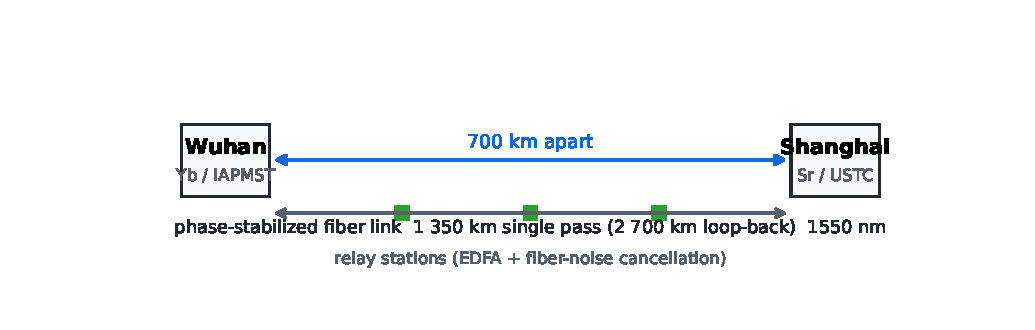
\includegraphics[width=\linewidth]{figs/fig1_network.pdf}
  \caption{The two-clock network. An IAPMST ytterbium clock in Wuhan and
  a USTC strontium clock in Shanghai are connected by a phase-stabilized
  \qty{1550}{nm} fiber link. Relay stations along the route carry
  erbium-doped fiber amplifiers and fiber-noise-cancellation loops.}
  \label{fig:network}
\end{figure}

Figure~\ref{fig:network} shows the two-clock network. An ytterbium (Yb)
lattice clock at IAPMST in Wuhan (systematic uncertainty
$\uYbE\times10^{-18}$~\citep{zhu2026yb}) and a strontium (Sr) lattice
clock at USTC in Shanghai ($\uSrE\times10^{-18}$~\citep{jia2026sr}) are
separated by $\siteKm$\,km and compared through a $\fibreKm$\,km
phase-stabilized fiber link ($\roundKm$\,km loop-back), with the
carrier transmitted from Shanghai to Wuhan on a \qty{1550.12}{nm}
telecom channel. The link extends the field-deployed link of
ref.~\citep{chen2026dissemination}, using the same cascaded
fiber-noise-cancellation technique; its added instability stays below
the clock noise for averaging times beyond $100$\,s.

Both combs are self-referenced and phase-locked to the local clock
signal, and all other frequencies in the chain derive from the two
clock transitions through fixed factor-of-two relations
(698/1397 nm on the Sr side; 578/1156 nm on the Yb side), so the two
clocks are the system's only independent frequency sources. The
recorded quantity is the out-of-loop beat between the received carrier
and the local Yb-referenced comb, sampled every second and converted to
fractional units with $F_{1550} = \fFifteenTHz$\,THz; the fiber
loop-back is monitored out of loop throughout. Each retained segment
yields a frequency-ratio estimate through the fixed frequency-chain
relations (see Methods).

Over two months (\nDays~days, \nStages~stages) the two clocks and their
transfer chains ran synchronously for a total of \nSamplesAll~valid
seconds, recorded as \nSegAll~jump-free segments; the data set analyzed
here comprises \nSeg~segments with \nSamples~seconds
(\nHours~effective hours). Figure~\ref{fig:campaign}a places the
segments on the campaign timeline.

\subsection{Clock-ratio determination}
\label{sec:results-ratio}

\begin{figure}[t]
  \centering
  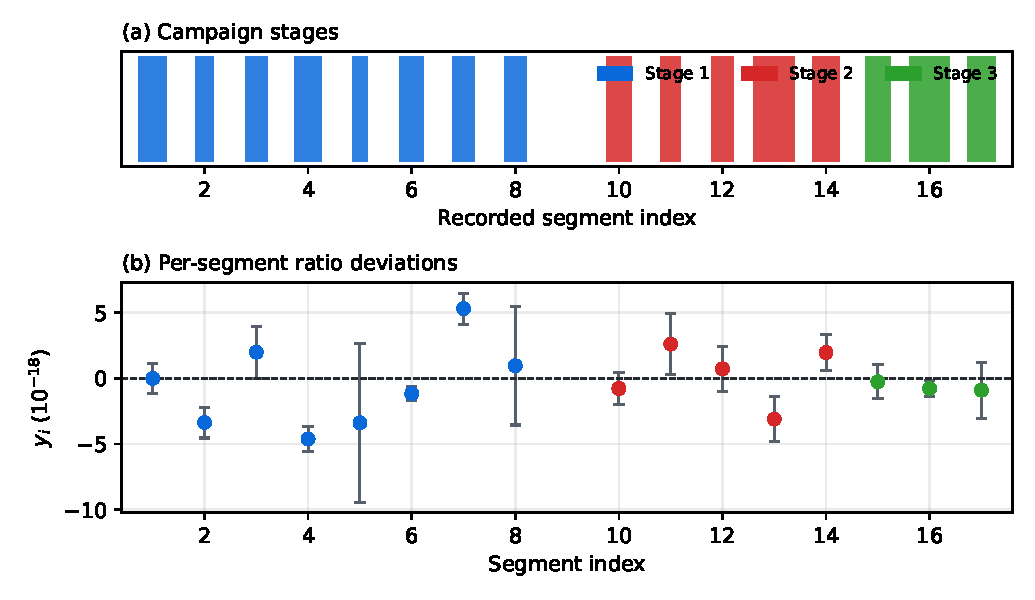
\includegraphics[width=\linewidth]{figs/fig2_campaign.pdf}
  \caption{Campaign and per-segment data. (a) Recorded segments colored
  by measurement stage; bar widths scale with the square root of the
  retained sample count. (b) Per-segment ratio deviations $y_i$ with
  their statistical uncertainties; the dashed line marks zero deviation.}
  \label{fig:campaign}
\end{figure}

We determine the Yb/Sr frequency ratio from the \nSeg~segments. Each
segment yields a ratio estimate with its own statistical uncertainty
estimated from the Allan deviation of the beat
(Methods). The segment estimates scatter more
than their individual uncertainties allow: the fixed-effect weighted
least-squares fit gives $\chi^2_{\rm red} = \chiRed$ for
$\dofV$ degrees of freedom ($p = \pChi$), and
\nModelLimited~of the \nSeg~segments have stability fits that fall
outside the white-frequency-noise band (groups \modelLimitedGroups).
We therefore adopt the Bayesian random-effect estimate, which treats
the excess scatter as a free parameter and propagates its posterior
uncertainty, while the fixed-effect WLS and Mandel--Paule estimates are
kept as cross-checks.

The resulting Yb/Sr ratio is
\begin{equation}
  \mathrm{Yb/Sr} = \Rheadline(\RheadlineUnc),
\end{equation}
with a statistical uncertainty of
$\uStatShort\times10^{-18}$ and a total standard uncertainty of
$\uTotalShort\times10^{-18}$ (Section~\ref{sec:results-budget}). The
precision-weighted cross-checks agree within their uncertainties:
the WLS center is \RwlsHead\xspace and the Mandel--Paule center is
\RmpHead\xspace (rounded at the 19th decimal), both consistent with
the adopted value at the $10^{-18}$ level. Figure~\ref{fig:campaign}b shows the per-segment
deviations; the segment-to-segment scatter is dominated by the
statistical noise of the individual segments and by the excess scatter
captured by the random-effect term.

\subsection{Uncertainty budget}
\label{sec:results-budget}

Table~\ref{tab:budget} collects the components of the total standard
uncertainty (Figure~\ref{fig:compare}b). The statistical term dominates
the budget, followed by the Yb and Sr systematic evaluations, the
static-potential term from the leveling, and the time-varying-redshift
term carried as an uncertainty item; the fiber-link and comb terms are
negligible at this precision. The total standard uncertainty is
$\uTotalShort\times10^{-18}$.

\begin{table}[t]
  \centering
  \caption{Uncertainty budget of the Yb/Sr frequency-ratio
  measurement. The time-varying gravitational-redshift term is carried
  as an uncertainty item and is not applied as a correction to the
  central value. Components are treated as independent.}
  \label{tab:budget}
  \begin{tabular}{lS[table-format=1.3]}
    \toprule
    Component & {Contribution ($10^{-18}$)} \\
    \midrule
    Statistical (Bayesian random effect) & \uStatE \\
    Sr systematics                       & \uSrE \\
    Yb systematics                       & \uYbE \\
    Static gravitational potential       & \uStaticE \\
    Fiber link                           & \uLinkE \\
    Frequency comb                       & \uCombE \\
    Time-varying redshift                & \uTidalE \\
    \midrule
    Total (quadrature)                   & \uTotalE \\
    \bottomrule
  \end{tabular}
\end{table}


% =====================================================================
\section{Discussion and outlook}
\label{sec:discussion}
% =====================================================================
The value reported here agrees with the two existing measurements of
the Yb/Sr ratio at the level set by the redefinition roadmap
(Figure~\ref{fig:compare}a). Relative to the NIST--JILA value
\refNistV(\refNistU)~\citep{aeppli2026nist}, our central value differs
by $\dVsNistE$; relative to the European-network value
\refEuV(\refEuU)~\citep{pizzocaro2026european}, it differs by
$\dVsEuE$. Both differences lie within the \refThreshold{} agreement
threshold of the roadmap's frequency-ratio
criterion~\citep{dimarcq2024roadmap, cctf2025taskforce}. To our
knowledge, this is the first reported intercity (100-km-scale),
cross-species frequency-ratio measurement meeting that uncertainty
requirement (as of \claimDate); existing ratios at or below the
threshold were measured on a single campus~\citep{aeppli2026nist},
while inter-institute comparisons through fiber networks have so far
reached \refEuBestU~\citep{pizzocaro2026european}. The result closes,
at intercity scale, the class of frequency-ratio measurements that
the SI-second redefinition process depends on. Meeting the roadmap's
frequency-ratio requirement has so far required clocks on a shared
campus, where a single stabilized link serves both systems; here the
two clocks sit in different cities, in different institutions, and use
different atomic species, and the measurement still reaches the
threshold, because the fiber link and the two combs contribute well
below the clocks themselves. The bottleneck for reaching the
redefinition threshold is therefore no longer the transfer
infrastructure but the systematic evaluations of the clocks and the
geodetic determination of their potential difference.

\begin{figure}[t]
  \centering
  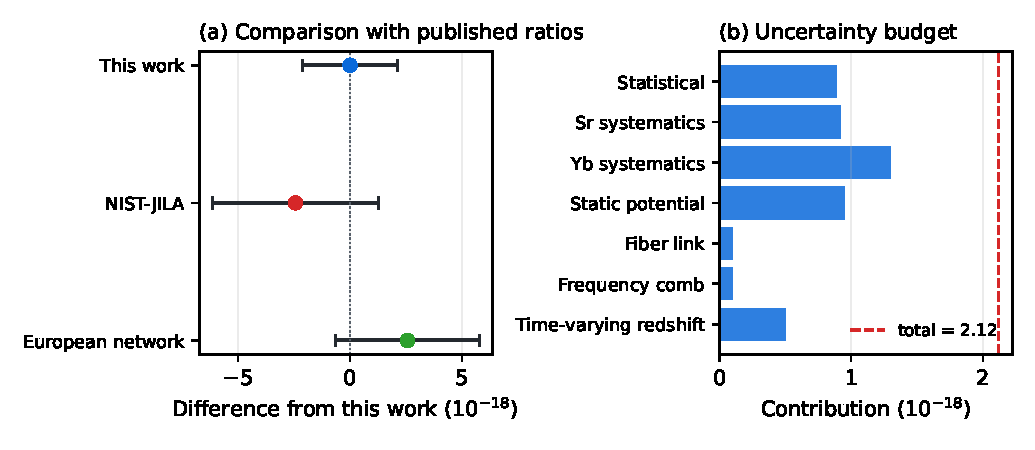
\includegraphics[width=\linewidth]{figs/fig3_compare.pdf}
  \caption{Comparison and budget. (a) Differences between this work and
  the published Yb/Sr ratios, with their quoted uncertainties.
  (b) Components of the total standard uncertainty; the dashed line marks
  the quadrature total.}
  \label{fig:compare}
\end{figure}

Changes in the Earth's gravitational potential enter the comparison
directly. The static difference between the two clock transitions is
fixed by first-order spirit leveling and is carried in the uncertainty
budget; of the time-varying contributions, the tidal term is carried as
a data-driven uncertainty item, while co-seismic steps from the
regional seismicity during the campaign fall well below the reported
precision. At this accuracy, it is the geodetic determination of the
potential difference, rather than its variability, that limits the
comparison; the same sensitivity underlies proposed
chronometric-geodesy applications of optical-clock
networks~\citep{grotti2018geodesy, takamoto2020redshift,
mcgrew2018geodesy}.

The campaign also demonstrates the operational character that a
future optical-clock network will need. Over the two-month campaign
the two clocks were restarted, the transfer chain re-locked, and the
beat record interrupted many times; the segment-level ratio estimates
show no evidence of a systematic offset between the three measuring
stages, so the reproducibility of the comparison does not depend on
continuous operation of either system. This is the practical
counterpart of the coordinated multi-clock
campaigns~\citep{lindvall2025coordinated, pizzocaro2026european}: the
network tolerates interruption, provided each retained window is
self-consistently characterized.

Several limitations bound the present result. First, the per-segment
statistical uncertainties from the Allan-deviation extrapolation are
the dominant budget term, and five of the sixteen segments carry
model-limited fits; the random-effect treatment accounts for their
excess scatter at the level of the reported uncertainty, but a longer
record would reduce the statistical term. Second, the systematic
evaluations of the two clocks are those published by the
laboratories; independent verification of those budgets, as opposed
to the transfer, is not attempted here. Third, the geopotential
difference is taken from a first-order leveling campaign; an
alternative value exists in the experiment records and is carried as
an external item pending reconciliation, as is the physical-model
provenance of the supplied tide series and the exact accounting of
the full sample totals. Finally, the present campaign meets the
uncertainty requirement of the roadmap but not the full criterion,
which additionally requires each ratio to be measured at least twice
by different institutes and repeated over an extended period.

Looking ahead, the result establishes this link as a prototype node
pair of a distributed optical-clock network: the same infrastructure
can be extended to further nodes, and the technique demonstrated here
-- clocks at different sites agreeing at the redefinition threshold --
is the operation that both the redefinition and post-redefinition
applications require. Realizing those applications over larger
distances will mean combining fiber networks of the kind used
here~\citep{schioppo2022cavities, chen2026dissemination} with
intercontinental techniques such as
VLBI~\citep{pizzocaro2021vlbi}, and will put the same demands on
geodetic infrastructure that this comparison
faced~\citep{grotti2018geodesy, mcgrew2018geodesy}.


% =====================================================================
% Nature layout: the reference list follows the main text, and the
% Methods section is the online-only apparatus (not numbered with the
% main text) placed after the reference list.
\bibliographystyle{unsrtnat}
\bibliography{refs}
% =====================================================================

\section*{Methods}
% =====================================================================
\subsection*{Experimental setup and frequency transfer}

The comparison links two optical lattice clocks at different institutions:
an ytterbium (Yb) clock at IAPMST in Wuhan and a strontium (Sr) clock at
USTC in Shanghai, about $\siteKm$\,km apart. The two sites are connected by
a phase-stabilized fiber link of $\fibreKm$\,km single-pass length
($\roundKm$\,km loop-back), operated at \qty{1550}{nm}. The route is
divided into spans of tens of kilometers, each terminated by a relay
station that carries a narrow-linewidth laser together with an
erbium-doped fiber amplifier and a fiber-noise-cancellation loop; the
added instability of the link is kept below the clock noise level for
averaging times beyond $100$\,s.

Both ends use independent optical frequency combs to bridge the
spectral gap between the clock transitions and the telecom carrier. On the
Shanghai side the Sr \qty{698}{nm} transition is transferred via a
\qty{1397}{nm} continuous laser to the \qty{1550}{nm} carrier; on the
Wuhan side the received carrier is linked to the Yb \qty{578}{nm}
transition through the \qty{1156}{nm} light. All local frequency
references and phase-locked loops are derived from the comb repetition
rate $f_{\mathrm{rep}} = \fRepMHz$\,MHz. The observable is the
out-of-loop beat between the received carrier and the local
Yb-referenced comb, converted to fractional units with the transfer
frequency $F_{1550} = \fFifteenTHz$\,THz (see Appendix~\ref{app:chain}).

\subsection*{Observation campaign and per-segment data}

The campaign spanned \nDays~days, from 29 June to 26 August 2026, in
\nStages~measurement stages. Synchronous-operation windows were first
defined from the lock status of the two clocks and of the beat signals;
within each window the longest continuous valid record was retained.
The selection used lock status only and did not refer to the resulting
ratio deviations. In total \nSegAll~jump-free segments were recorded,
carrying \nSamplesAll~valid seconds; the data set analyzed here
comprises \nSeg~segments with \nSamples~valid seconds
(\nHours~effective hours).

\subsection*{Clock-ratio determination and statistical model}

Each retained segment yields a clock-ratio estimate $R_i$ from the mean
of its retained beat samples, inverted through the fixed frequency-chain
relation (Appendix~\ref{app:chain}) and corrected for the static
gravitational redshift $\delta_g = \deltaGV$ derived from the leveled
geopotential difference (see below). The
per-segment statistical uncertainty $u_i$ is obtained from the
overlapping Allan deviation of the beat fractional frequency: a
$\sigma_y \propto \tau^{-1/2}$ fit over the range
$128~\mathrm{s} \le \tau \le 0.25\,T_i$, extrapolated to the segment
duration $T_i$.

The per-segment uncertainties do not fully explain the observed scatter
between segments, so the ratio is combined with four estimators:
fixed-effect weighted least squares (WLS, weights $1/u_i^2$), Birge
scaling, the Mandel--Paule random-effect model, and a Bayesian
random-effect model in which the excess scatter $\xi$ is a free
parameter whose posterior uncertainty is propagated into the final
result. The Bayesian random-effect center is adopted as the primary
statistic; the others are reported as cross-checks. Five of the
\nSeg~segments (groups \modelLimitedGroups) have stability fits that
fall outside the white-frequency-noise band and are carried with a
model-limited flag; this is one motivation for the random-effect
treatment. The full model definitions are given in
Appendix~\ref{app:stats}.

\subsection*{Leveling determination of the geopotential difference}

The static gravitational-redshift correction is fixed by the
geopotential difference between the two clocks' atomic transition
positions, determined by first-order spirit leveling together with
simultaneous gravimetry. A leveling line of about $\levelKm$\,km was
run between the Wuhan benchmark WS-03 (at IAPMST) and the Shanghai
benchmark WS-01 (at USTC) through Ezhou, Huangshi, Huanggang, Lu'an,
Hefei, Wuhu, Guangde and Suzhou, using digital levels with sight
lengths below \qty{30}{m} and gravity observed at every leveling point
with two relative gravimeters. The leveled normal heights were
converted to orthometric heights for the geopotential integration,
$\dW_{AB} = -\sum_i g_i\,\Delta H_i$, where $g_i$ is the mean gravity
and $\Delta H_i$ the orthometric height difference of the $i$-th
segment. The resulting geopotential difference between the two atomic
transitions is $\dW = \dWVal \pm \dWUnc~\mathrm{m^2\,s^{-2}}$. The
per-kilometer misclosure of the leveling is $\levelMm$\,mm, below the
first-order limit.

\subsection*{Uncertainty budget}

Table~\ref{tab:budget} lists the uncertainty components of the
Yb/Sr ratio. The statistical term is the posterior standard deviation
of the Bayesian random-effect model applied to the \nSeg-segment data.
The Sr and Yb systematic terms are the published evaluations of the two
clocks~\citep{jia2026sr, zhu2026yb}; the value adopted for the Yb clock
resolves an internal-versus-published discrepancy in favor of the
published evaluation. The static-potential term follows from the
leveling uncertainty. The fiber-link and frequency-comb terms are
experiment-side upper bounds. The time-varying
gravitational-redshift term is carried as an uncertainty item,
quantified from the scale over which the segment-averaged shift varies
across the campaign, and is not applied as a correction to the reported
central value. The components are treated as independent and combined
in quadrature.


% =====================================================================
\section*{Data availability}
% =====================================================================
The frozen, machine-readable result layer underlying this manuscript is
archived in the repository
(\url{https://github.com/hjiang555-a11y/gravitation-whsh}) under
\texttt{results/audit-v1/verified/}: the manifest with SHA-256
\texttt{15725f5246e87af5a450c8e31ccf0d0ef277d517a493ed1fb44d65a4b86564d4},
the derived ledgers and statistics, and the generated audit report. The raw
beat files and the leveled geopotential inputs are not redistributed.

% =====================================================================
\section*{Code availability}
% =====================================================================
The analysis and manuscript pipelines are in the same repository under the
Apache License 2.0. The manuscript numbers are generated by
\texttt{paper/rev2/tools/build\_numbers.py}, which reads only the frozen
manifest and the curated constants listed in
\texttt{generated/numbers\_manifest.json}.

% =====================================================================
\appendix
\section{Frequency chain and ratio inversion}
\label{app:chain}

The observable is the out-of-loop beat between the transferred
\qty{1550}{nm} carrier and the local Yb-referenced comb. All
frequencies in the chain derive from the comb repetition rate
$f_{\mathrm{rep}} = \fRepMHz$\,MHz. The Sr clock's absolute frequency
$f_{\mathrm{Sr}}$ (\qty{698}{nm}) is related to the comb frequency fed
to the \qty{1397}{nm} branch by
\begin{equation}
  f_{\mathrm{comb}}^{1397} = \tfrac{1}{2}\,(1 + a)\,f_{\mathrm{Sr}},
\end{equation}
where $a$ collects the Sr systematic corrections (density, lattice,
second-order Zeeman and BBR shifts). The Yb clock's absolute frequency
$f_{\mathrm{Yb}}$ (\qty{578}{nm}) relates to the \qty{1156}{nm} comb
branch by
\begin{equation}
  f_{\mathrm{comb}}^{1156} = \tfrac{1}{2}\,(1 + b)\,f_{\mathrm{Yb}}.
\end{equation}
The beat is converted to fractional units with the transfer frequency
$F_{1550} = \fFifteenTHz$\,THz. The static gravitational-redshift
correction enters the ratio inversion as a multiplicative factor,
\begin{equation}
  \left(\mathrm{Yb/Sr}\right)_{\rm corr}
  = \left(\mathrm{Yb/Sr}\right)_{\rm raw} \times (1 + \delta_g),
  \qquad \delta_g = \deltaGV,
\end{equation}
derived from the leveled geopotential difference
$\dW = \dWVal \pm \dWUnc~\mathrm{m^2\,s^{-2}}$ (Methods).

\section{Data processing and segment definition}
\label{app:processing}

The counters sample the beat every second in phase-averaging mode.
Samples deviating by more than $10$\,Hz from the running median are
treated as jump points and removed; the retained data are further
trimmed at both ends by an endpoint screen that drops points beyond
$1\%$ of the peak-to-peak range of the record. The data set analyzed
here consists of the longest jump-free record of each accepted segment
after this screening. Table~\ref{tab:segments} lists the per-segment
retained counts, ratio deviations and statistical uncertainties; the
category column marks the five segments whose stability fits are
model-limited.

\begin{table}[t]
  \centering
  \caption{Per-segment data of the 16 segments analyzed in this work. Ratio
  deviations $y_i = R_i/R_1 - 1$ are relative to the first segment;
  $u(y_i)$ is the statistical uncertainty of the segment ratio;
  ``Fit'' is \emph{est.} for segments whose stability fit lies in the
  white-frequency-noise band and \emph{lim.} for model-limited fits.}
  \label{tab:segments}
  % Generated by tools/build_numbers.py -- do not edit by hand.
\begin{tabular}{rrrrl}
\toprule
Group & $n_{\rm valid}$ & $y_i$ ($10^{-18}$) & $u(y_i)$ ($10^{-18}$) & Fit \\
\midrule
1 & 68\,009 & +0.00 & 1.113 & est. \\
2 & 29\,481 & -3.36 & 1.178 & lim. \\
3 & 42\,891 & +2.00 & 1.984 & est. \\
4 & 64\,280 & -4.61 & 0.951 & est. \\
5 & 19\,532 & -3.38 & 6.040 & est. \\
6 & 52\,140 & -1.15 & 0.513 & lim. \\
7 & 39\,526 & +5.31 & 1.173 & lim. \\
8 & 43\,565 & +0.97 & 4.509 & est. \\
10 & 57\,938 & -0.76 & 1.230 & est. \\
11 & 35\,824 & +2.61 & 2.301 & est. \\
12 & 40\,346 & +0.73 & 1.715 & lim. \\
13 & 152\,994 & -3.09 & 1.694 & est. \\
14 & 68\,618 & +1.97 & 1.377 & est. \\
15 & 57\,649 & -0.25 & 1.293 & est. \\
16 & 147\,640 & -0.77 & 0.607 & lim. \\
17 & 65\,983 & -0.89 & 2.142 & est. \\
\bottomrule
\end{tabular}

\end{table}

\section{Statistical combination models}
\label{app:stats}

\paragraph{Fixed-effect WLS.} Under the assumption that all segments
estimate one common ratio with uncertainties $u_i$,
\[
  \mu_{\rm WLS} = \frac{\sum_i w_i R_i}{\sum_i w_i}, \quad
  w_i = 1/u_i^2, \quad
  u_{\rm WLS} = \left(\sum_i w_i\right)^{-1/2},
\]
with $\chi^2 = \sum_i (R_i - \mu_{\rm WLS})^2 / u_i^2$ and
$\chi^2_{\rm red} = \chi^2/(N-1)$. For the analyzed data set,
$\chi^2_{\rm red} = \chiRed$ ($N = \nSeg$,
$\dofV$ degrees of freedom, $p = \pChi$), so the fixed-effect
uncertainty under-describes the observed scatter.

\paragraph{Birge scaling.} The Birge ratio
$B = \sqrt{\chi^2_{\rm red}} = \birgeRatio$ scales all segment
uncertainties by a common factor, $u_i \to B u_i$; it assumes the
relative sizes of the $u_i$ are correct but their overall scale is
not.

\paragraph{Mandel--Paule.} An excess scatter $\xi$ common to all
segments is added in quadrature, $u_{i,\rm eff}^2 = u_i^2 + \xi^2$,
and $\xi$ is solved from $\chi^2_{\rm red}(\xi) = 1$. For the analyzed
data set, $\xi = \xiMpE \times 10^{-18}$.

\paragraph{Bayesian random effect.} The same observation model,
$R_i \sim \mathcal{N}(\mu, u_i^2 + \xi^2)$, is treated
hierarchically: $\mu$ and $\xi$ are both inferred, with flat priors
on $\mu$ and on $\log\xi$, and the joint posterior
$p(\mu, \xi \mid \{R_i, u_i\})$ is marginalised numerically over a
40-decade log-$\xi$ grid. The reported central value is the posterior
mean of $\mu$ and the statistical uncertainty is its posterior
standard deviation; for the analyzed data set,
$\xi = \xiBayesE \times 10^{-18}$. The excess scatter quantified here
also absorbs the correlated component of the time-varying
gravitational-redshift term (Methods), which
is carried separately as an uncertainty item rather than corrected.

\section{Leveling reduction}
\label{app:leveling}

The orthometric height difference between benchmarks follows from the
leveled normal heights after the normal-to-orthometric conversion,
with gravity observed at every leveling point. The geopotential
difference is integrated segment by segment,
$\dW_{AB} = -\sum_i g_i \Delta H_i$, and combined with the two local
offsets between benchmark and clock platform (obtained by
trigonometric leveling) and the platform-to-transition offsets from
the clock design parameters. The resulting atomic-transition
geopotential difference is $\dW = \dWVal \pm \dWUnc~\mathrm{m^2\,s^{-2}}$,
equivalent to an optical fractional shift of $\deltaGV$.

\section{Uncertainty budget details}
\label{app:budget}

The components of Table~\ref{tab:budget} are obtained as follows.
The statistical term is the posterior standard deviation of the
Bayesian random-effect model (Appendix~\ref{app:stats}). The Sr and
Yb terms are the published systematic uncertainties of the two
clocks~\citep{jia2026sr, zhu2026yb}; for the Yb clock the published
evaluation is adopted. The static-potential term is
$u(\dW)/c^2$ from the leveling uncertainty
$\dWUnc~\mathrm{m^2\,s^{-2}}$, giving
$\uStaticE \times 10^{-18}$. The fiber-link and comb terms are
experiment-side upper bounds of $\uSubsystemBound$ each, carried at
\uLinkE $\times 10^{-18}$ and $\uCombE \times 10^{-18}$ to preserve the
experiment-side margin. The time-varying-redshift term is scaled from
the spread of the segment-averaged gravitational shift across the
campaign and is carried at $\uTidalE \times 10^{-18}$; it is not
applied as a correction. The total standard uncertainty,
$\uTotalE \times 10^{-18}$, is the quadrature sum of the seven
components.

% =====================================================================

\end{document}
